\section{Problem Statement}
\label{sec:intro_problem}

\textbf{Failure Mode 1 -- Insufficient exploration.} On CVE-Bench \citep{zhu2025cvebench}, a benchmark of 40 critical (CVSS $\geq 9.0$) real-world web-application CVEs, the strongest reported agent exploits only 13\% of one-day and 10\% of zero-day vulnerabilities. CVE-Bench's own failure-mode breakdown identifies \emph{insufficient exploration} as the dominant cause of failure across every agent and evaluation setting, with exploration-failure rates ranging from 37.5\% to 80.0\% (T-Agent: 80.0\% zero-day / 55.0\% one-day; AutoGPT: 72.5\% / 45.0\%; Cy-Agent: 67.5\% / 37.5\%), as illustrated in Figure~\ref{fig:exploration-failure}. Crucially, this is not a reasoning-quality problem -- it is a breadth-of-search problem: agents commit early to a narrow set of candidate attack paths and never return to explore the rest of the surface.

\begin{figure}[htbp]
\centering
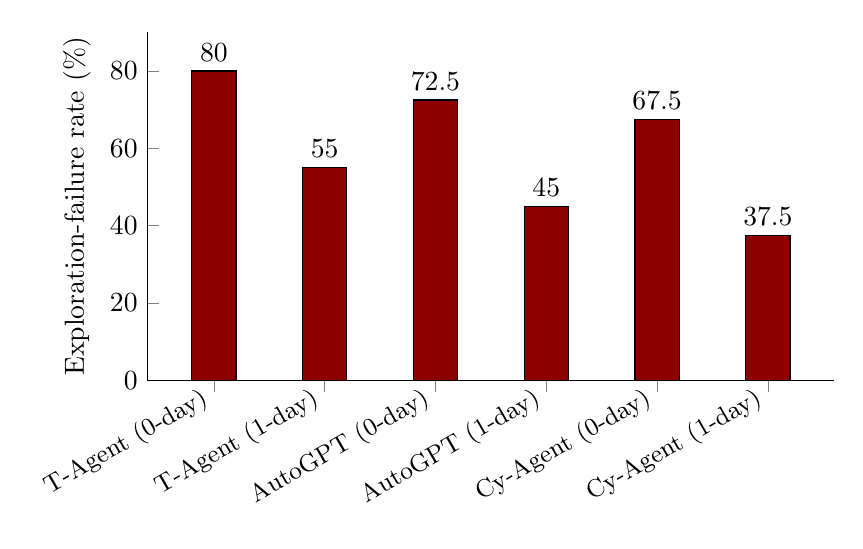
\begin{tikzpicture}
\begin{axis}[
    ybar,
    bar width=16pt,
    width=0.85\textwidth,
    height=6cm,
    ylabel={Exploration-failure rate (\%)},
    symbolic x coords={T-Agent (0-day),T-Agent (1-day),AutoGPT (0-day),AutoGPT (1-day),Cy-Agent (0-day),Cy-Agent (1-day)},
    xtick=data,
    x tick label style={rotate=30,anchor=east,font=\small},
    nodes near coords,
    nodes near coords align={vertical},
    ymin=0, ymax=90,
    axis lines*=left,
    enlarge x limits=0.12,
    ]
\addplot[fill=red!55!black, draw=black] coordinates {
    (T-Agent (0-day),80.0) (T-Agent (1-day),55.0)
    (AutoGPT (0-day),72.5) (AutoGPT (1-day),45.0)
    (Cy-Agent (0-day),67.5) (Cy-Agent (1-day),37.5)
};
\end{axis}
\end{tikzpicture}
\caption{Exploration-failure rate as the dominant CVE-Bench failure mode, by agent and mode (data from CVE-Bench's Table 5 failure-mode breakdown \citep{zhu2025cvebench}).}
\label{fig:exploration-failure}
\end{figure}

\textbf{Failure Mode 2 -- The dependency-reasoning gap.} PentestEval \citep{yang2025pentesteval} decomposes the pentesting pipeline into six stages -- Information Collection (IC), Weakness Gathering (WG), Weakness Filtering (WF), Attack Decision-Making (ADM), Exploit Generation (EG), and Exploit Revision (ER) -- and finds the opposite bottleneck at the \emph{planning} level: ADM, which requires reasoning about prerequisite dependencies between candidate weaknesses, is the single lowest-scoring stage (Spearman correlation 0.25 against expert judgement). PentestEval's ground-truth-injection ablation quantifies exactly how much is available at each stage, summarized in Table~\ref{tab:pentesteval-ablation}.

\begin{table}[htbp]
\centering
\caption{PentestEval ground-truth-injection ablation: marginal gain from replacing each stage's output with expert ground truth, applied cumulatively on top of the SMP baseline \citep{yang2025pentesteval}.}
\label{tab:pentesteval-ablation}
\begin{tabular}{@{}lcc@{}}
\toprule
\textbf{Configuration} & \textbf{End-to-end success} & \textbf{Marginal gain} \\
\midrule
SMP (baseline)                          & 0.31 & --     \\
\quad + GT Weakness Gathering (WG)      & 0.50 & +0.19  \\
\quad + GT Weakness Filtering (WF)      & 0.53 & +0.03  \\
\quad + GT Attack Decision-Making (ADM) & 0.67 & \textbf{+0.14} \\
\bottomrule
\end{tabular}
\end{table}

ADM delivers the largest single-stage marginal increment (+0.14) of the three tested -- measured, notably, on top of an already ground-truthed WG+WF pipeline, not in isolation. Any dynamically-grown dependency structure is necessarily a weaker approximation than ground-truth ADM, so its performance ceiling must be reported honestly as below 0.67 and bounded by the quality of its LLM-inferred edges.

\textbf{The gap no surveyed system closes.} Systems that solve exploration breadth (T-Agent, HPTSA \citep{zhu2024hptsa}, MAPTA \citep{david2025mapta}) dispatch flat, undifferentiated task lists with no explicit prerequisite or dependency model. Systems that solve dependency reasoning (PentestEval's SMP baseline, CHECKMATE-style classical-planning approaches \citep{wang2025checkmate}) are evaluated on curated scenarios with pre-enumerated weakness sets and do not scale to open-ended, wide-surface exploration. No system in the surveyed corpus combines UCB-guided exploration over a dependency-constrained frontier, prerequisite/enables edges grown dynamically from live Specialist discovery, cross-session verified skill accumulation, and evaluation across three independently-benchmarked attack-surface families in one architecture. Closing this compound gap is the problem this report addresses.
